\documentclass[tikz,border=8pt]{standalone}
\usepackage[T1]{fontenc}
\usepackage{amsmath,amssymb,newtxtext,newtxmath}
\usetikzlibrary{arrows.meta,decorations.markings,patterns,calc}
\definecolor{ink}{HTML}{20364D}
\definecolor{accent}{HTML}{287B83}
\definecolor{wash}{HTML}{EEF5F6}
\definecolor{warm}{HTML}{A24D38}
\begin{document}
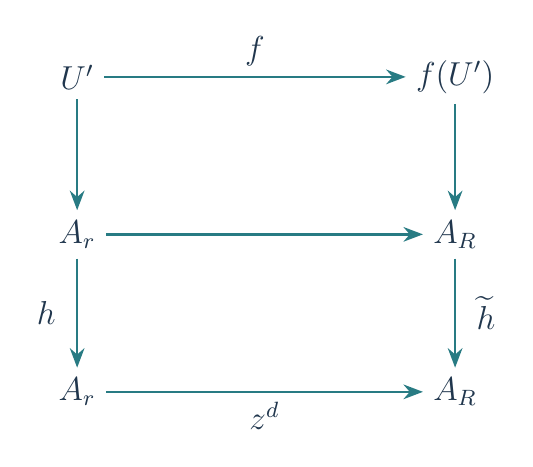
\begin{tikzpicture}[font=\large,text=ink,draw=ink,line width=.8pt,
  arr/.style={-Stealth,draw=accent,line width=.9pt},
  lab/.style={inner sep=2pt},
  region/.style={draw=ink,fill=wash},
  pt/.style={circle,fill=ink,inner sep=1.6pt}]
% Source page 14: annular maps. The arbitrary map and its lift use the
% notation restored in the accompanying manuscript passage.
\node (a) at (0,0) {$U'$}; \node (b) at (4.8,0) {$f(U')$};
\node (c) at (0,-2) {$A_r$}; \node (d) at (4.8,-2) {$A_R$};
\node (e) at (0,-4) {$A_r$}; \node (g) at (4.8,-4) {$A_R$};
\draw[arr] (a)--node[above] {$f$} (b);
\draw[arr] (a)--(c); \draw[arr] (b)--(d);
\draw[arr] (c)--(d);
\draw[arr] (c)--node[left=4pt] {$h$} (e);
\draw[arr] (d)--node[right=4pt] {$\widetilde h$} (g);
\draw[arr] (e)--node[below] {$z^d$} (g);
\end{tikzpicture}
\end{document}
